From our full sample of 166 stars, \rev{102} age posteriors are based on lithium upper limits alone, while \rev{55} stars have an age posterior based on more than one tracer. \rev{31} of our targets ($\sim19\%$) have a median age younger than 1 Gyr, which is more than expected for a uniform star formation rate. We discuss the full age distribution of our sample below.

\subsection{Star Formation History of the Solar Neighborhood}

 \cite{1990Ap&SS.163..229R} and \cite{2023MNRAS.522.1643C} found that the local star formation rate has been near constant for the last 10 to 12 Gyr based on the luminosity distribution of white dwarfs. Other studies found slightly different histories: a maximum star formation rate ($\sim2$ times the typical star formation rate at other times) $\sim3$ Gyr ago \citep{2006A&A...459..783C} or two star forming events separated by $\sim5$ Gyr \citep{2018Natur.559..585N}.  We assume a uniform star formation history, which also matches the priors used in \texttt{BAFFLES} \citep{2020ApJ...898...27S} and \texttt{gyro-interp} \citep{2023ApJ...947L...3B}.

\subsection{Population Level Ages}

\rev{We investigate how significant it is that our sample contains more stars than expected with median ages younger than 1 Gyr. Given the small size of our sample ($<200$ stars), and the biased nature in which it was selected, we are not attempting here to constrain the local star formation history. Rather, we are examining whether the total age distribution we observe is broadly consistent with a uniform star formation rate in the solar neighborhood.} We construct a population-level age distribution by summing (and then normalizing) the age posteriors for the entire sample. This is equivalent to marginalizing over individual stars; in the limit where each age posterior is a delta-function, this method produces a histogram of stellar ages. With a large enough volume-limited sample, we would expect this population-level distribution to match the star formation of the solar neighborhood. \rev{If the star formation rate has been uniform from 0 to 13 Gyr, we expect 1/13 ($7.7\%$) of the summed age distribution  to be younger than 1 Gyr.}

The left panel of Figure \ref{global_post} shows the population-level age distribution for our 166-star sample, which peaks at young ages ($\lesssim$2 Gyr). Part of this peak is due to early-type stars, which have short main sequence lifetimes and thus do not trace the full 13 Gyr star formation history. These stars make up $\sim19\%$ of the sample which is an over-representation relative to the initial mass function \citep{1955ApJ...121..161S, 2003PASP..115..763C, 2003ApJ...598.1076K}. This is likely due to the multiplicity fractions ($\sim50-70\%$) of these stars \citep{2023ASPC..534..275O} making them more likely to be accelerating. Removing stars with $B-V < 0.595$ (corresponding to a main sequence mass of $1.06 \ M_{\odot}$) \rev{leaves us with 135 stars and} produces the posterior in the right panel of Figure \ref{global_post}. The peak at young ages is still present, but less pronounced. 

 

\begin{figure*}[ht!]
\centering
 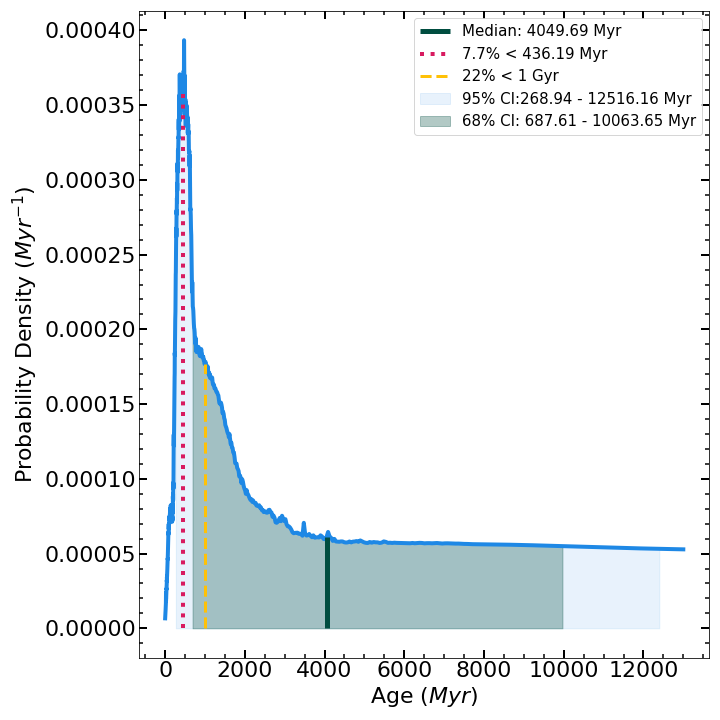
\includegraphics[scale = 0.35]{global_post.png}
 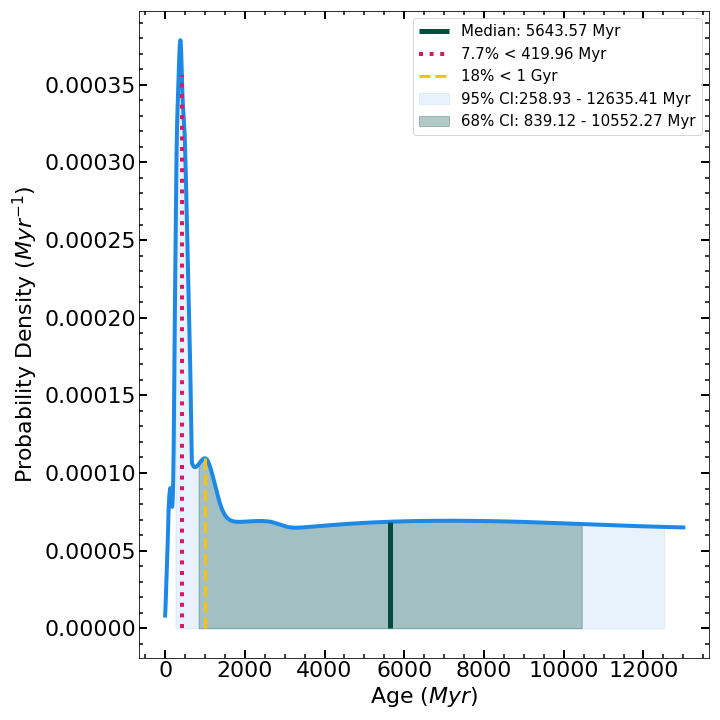
\includegraphics[scale = 0.35]{global_post_late.png}
 \caption{{\bf Left}: Sum of all the age posteriors for the full sample. The distribution of ages is peaked at young ages, but this is partially due to the inclusion of early-type stars with shorter main sequence lifetimes. {\bf Right}: Sum of age posteriors for only stars with $B-V > 0.595$, where there is still a peak at young ages, if less pronounced than for the full sample.}
 \label{global_post}
\end{figure*}

This general behavior is consistent with the types of age posteriors we produce here. For any given late-type star the posterior is either a well-constrained Gaussian-like peak or a lower age limit (corresponding to a lithium upper limit) with only the youngest ages ruled out. While $R^{'}_{HK}$ produces Gaussian-like posteriors at both young and old ages for stars earlier than K2, lithium and gyrochronology generally produce peaked posteriors for later spectral types if they are younger than $\sim$1 Gyr. Stars older than $\sim$1 Gyr mostly do not have detectable lithium (depending on spectral type), and either have rotation periods longer than a typical  $TESS$ sector or are less spotted. \rev{For the reduced sample of 135 stars, we expect $\sim10$ ($7.7\%$) stars to be younger than 1 Gyr. Following the Poisson distribution, we calculate a $65\%$ chance of between 8 and 13 stars being younger than 1 Gyr and a $96\%$ chance of between 5 and 17 stars being younger than 1 Gyr. Testing this prediction is complicated by the fact that we have somewhat broad age posteriors, rather than delta-function age measurements. Nevertheless, we can estimate the number of young stars in our sample by summing the probability in the posteriors for all stars. We calculate that $18\%$ of the age posterior for the reduced sample falls below 1 Gyr. This corresponds to $\sim24$ stars, which is significantly higher than expected. In fact, for a Poisson distribution with an expectation value of 10.4 stars, we only expect a value of 24 or higher $0.01\%$ of the time.}


%In Figure \ref{global_post}, it is clear that the distribution of ages for our sample is not as uniform as expected given the assumed constant star formation rate in the solar neighborhood. Even after removing the early-type stars that are over-represented in the sample and are therefore partially responsible for skewing the distribution towards younger ages, there remains an extreme peak at ages $\lesssim1$ Gyr. 

\subsection{Testing Individual Age Tracers}

Figure \ref{global_post_late} further divides the late spectral type stars. The left panel only includes posteriors from lithium detections and/or rotation period detections. The right panel only includes posteriors derived from lithium upper limits. The posterior derived exclusively from lithium upper limits, as expected, is much less peaked and is essentially following the prior. The posterior derived from lithium detections and rotation rates peaks at ages younger than $\sim$1 Gyr. This peaked posterior is expected for age tracers that only return peaked posteriors for the youngest stars.


\begin{figure*}[ht!]
\centering
 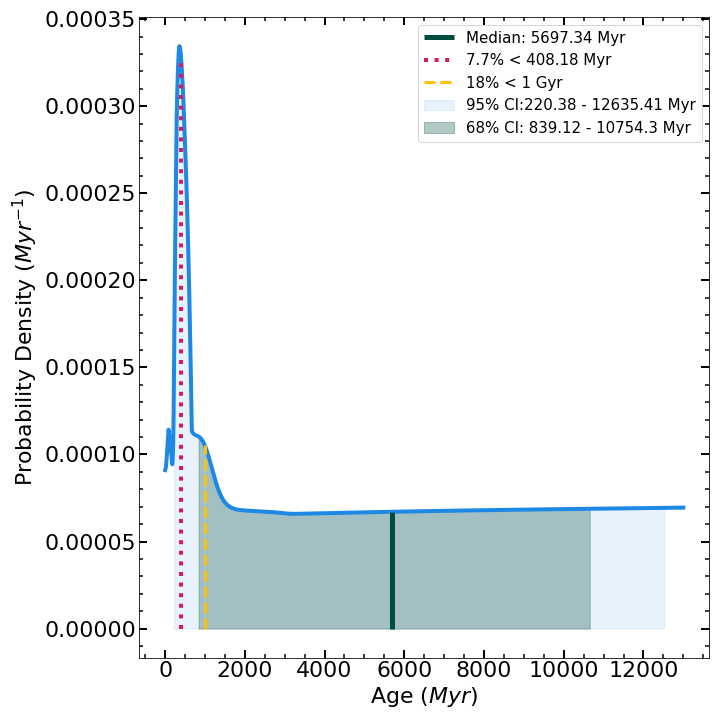
\includegraphics[scale = 0.35]{global_post_late_lid_gyro.png}
 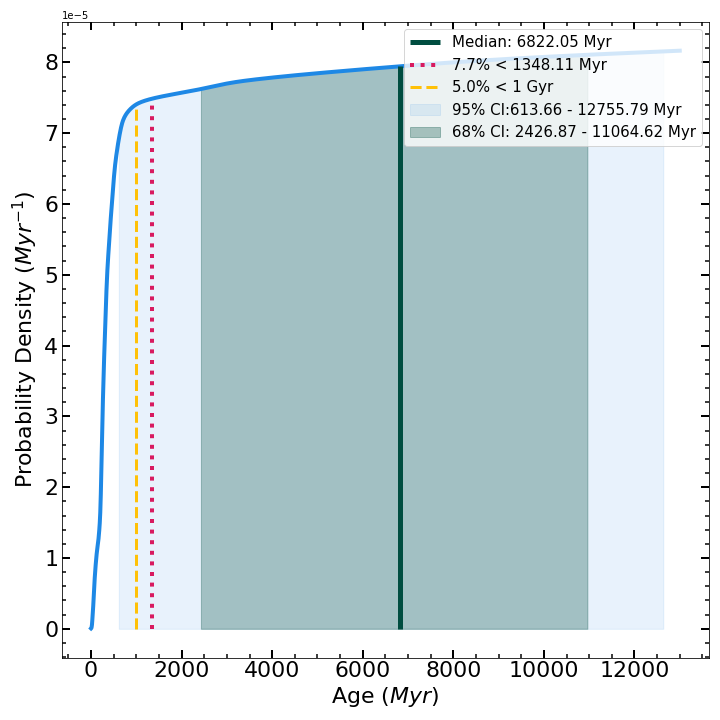
\includegraphics[scale = 0.35]
 {global_post_late_Li_UL.png}

 \caption{{\bf Left}: The combined age posterior from lithium detections and/or gyrochronology for the late-type stars in the sample. The peak at young ages is consistent with stars that are $<1$ Gyr being most likely to have detectable lithium or clear rotation signals. {\bf Right}: For stars that only have lithium upper limits, the age posterior is mostly flat, following the prior, with only the youngest ages excluded.}
 \label{global_post_late}
\end{figure*}


\rev{Nevertheless, this peak seems to include more probability at ages less than 1 Gyr than we would expect from a uniform star formation rate operating between 0 and 13 Gyr. We investigate the relative contributions of lithium and gyrochronology to this result in Figure \ref{LiGyroPost}. We consider ages from lithium, calcium, and gyrochronology separately. }

\rev{{\bf Lithium}: We find that the combined age posterior for lithium-only derived posteriors (114 posteriors) is consistent with a uniform star formation rate. From the Poisson distribution and an assumed uniform star formation rate history, there is an $82\%$ chance of  between $5\leq N_{stars} \leq 11$ being younger than 1 Gyr. We calculate $8.0\%$  of the posterior ($\sim9$ stars) falls below 1 Gyr, consistent with this prediction.} 

\rev{{\bf Calcium}: We derive age posteriors from $R^{'}_{HK}$ for 18 late-type stars. There are 7 additional late-type stars that have appropriate $B-V$ values to derive posteriors from $R^{'}_{HK}$ but have $R^{'}_{HK} \leq -5$, which is outside the calibration range of \texttt{BAFFLES}, but consistent with old ages. From the Poisson distribution, there is a $\sim60\%$ chance of measuring between 0 and 1 stars younger than 1 Gyr from a sample of 18 stars. $1\%$ of our 18 star $R^{'}_{HK}$ posterior falls below 1 Gyr, which corresponds to finding $0.18$ stars being less than 1 Gyr, which is again consistent with the prediction.} 

\rev{{\bf Gyrochronology}: We have  $TESS$ light curves for 129 stars, 106 of which have $B-V > 0.595$. We measure rotation periods for 20 of the late-type stars. From the gyrochronology population-level age distribution, $92\%$ of the probability is less than 1 Gyr, which corresponds to $\sim17\%$ of the total late-type gyrochronology sample of 106 stars, or about 18 young stars. Our ages from gyrochronology do not include upper limits because flat  $TESS$ light curves could indicate a long rotation period (longer than a typical  $TESS$ sector) or just a star without significant star spots. Overall, we would expect $\sim8$ stars out of 106 to have an age of 1 Gyr or younger. From the Poisson distribution with an expectation value of 8, there is a $\sim4\%$ chance of finding 13 or more stars below 1 Gyr, and a $\sim0.08\%$ chance of finding 18 or more. Thus, while the number of young stars identified from lithium and calcium alone are consistent with the predictions of a uniform star formation rate,  there appears to be $\sim5-10$ excess young stars identified by rotation. 

This result, that our combined age posterior suggests 18.0 stars are younger than 1 Gyr, does not change significantly even if we increase the size of the rotational period errors when computing age posteriors. Our period errors are between 0.11 days and 2.02 days, with a median of 0.55 days. Setting a minimum error bar to 1 day, 2 days, or 3 days still results in an estimate that 18.4, 17.8, and 16.8 stars are younger than 1 Gyr, respectively. As a result, we conclude that this excess of probability at young ages cannot be attributed solely to a systematic underestimate of the rotation period uncertainties.


\begin{figure*}[ht!]
\centering
 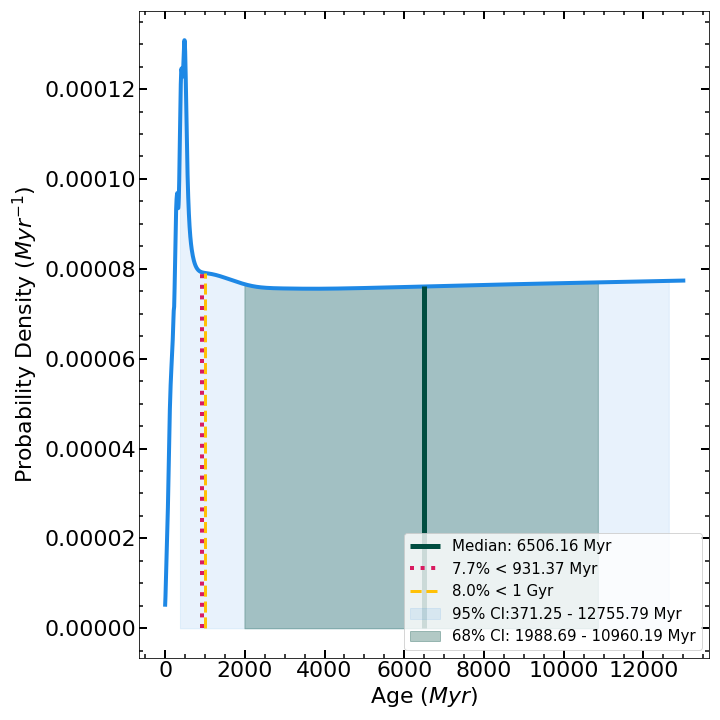
\includegraphics[scale = 0.35]{global_post_late_Li.png}
  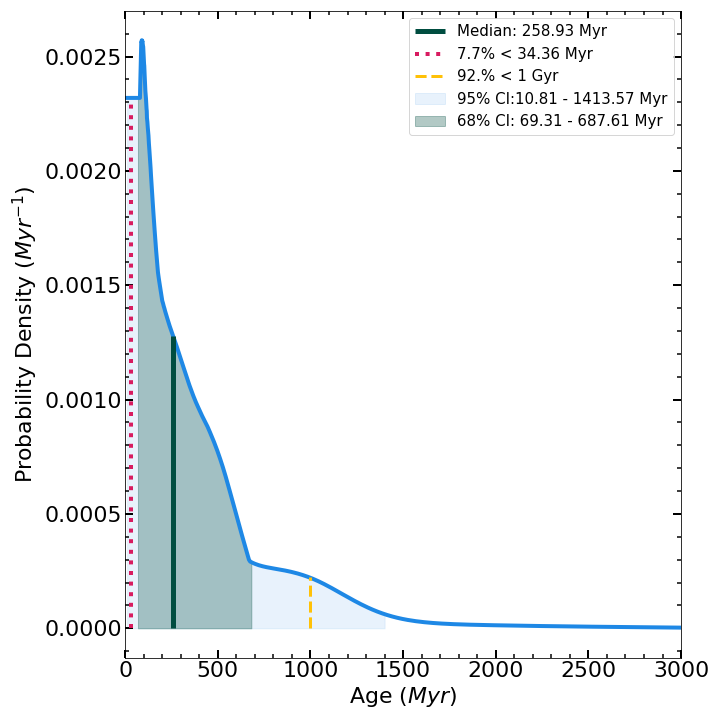
\includegraphics[scale = 0.35]{global_post_late_Gyro.png}
 

 \caption{{\bf Left:} Ages derived from lithium alone yield an age distribution consistent with a constant star formation rate. $8\%$ of the combined distribution falls below 1 Gyr, which is consistent with the expected $7.7\%$. {\bf Right:} Ages derived from gyrochronology alone yield a significantly younger age distribution than expected. For the \rev{20} late-type stars with rotation periods $\lesssim15$ days, $92\%$ of the combined distribution of ages falls below 1 Gyr, which corresponds to \rev{$\sim17\%$} of the full gyrochronology sample.}
 \label{LiGyroPost}
\end{figure*}

There are several possible explanations for the higher-than-expected fraction of young stars in the gyrochronological sample. Since we select stars that are accelerating, there is a greater chance of selecting a short-period stellar binary \rev{(e.g. \citealt{2019AJ....158..226D})}. The rotational evolution of stars in close binaries could be influenced by tides resulting in shorter rotation periods than expected from age alone. Additionally,  $TESS$ pixels may be contaminated by multiple stars (either physical binaries or crowded fields). While we screen for contaminated pixels, additional components may be present in some light curves. Alternatively, this effect could be physical: if binaries become unbound over time, a sample of accelerating stars (which is more likely to contain binaries than the field) would be younger than a volume-limited sample.

While we screened our initial accelerating star sample for binaries from WDS, SB9, and archival imaging, such a search is not complete to all binary configurations. Indeed, by constructing our sample from accelerating stars not in these catalogs we expect undiscovered binaries to be overrepresented in our sample compared to an unbiased volume-limited sample. For example, three eclipsing binaries (HIP 16247, HIP 45731, and HIP 49577) discussed in Section \ref{sec:gyro} were discovered to be physical binaries only after our survey began. We are currently carrying out radial velocity monitoring of the full sample with the aim of identifying additional short-period stellar binaries, and will report the results in a future paper.}

 
\rev{\subsection{Companions}
Since the beginning of this survey in 2020, two brown dwarf companions have been discovered around two of the accelerating stars discussed in this work. \cite{2022ApJ...934L..18K} found a $\sim28  \ M_\textrm{Jup}$ companion to HIP 21152, a likely member of the Hyades Cluster ($\sim750$ Myr; \rev{\citealt{2018ApJ...856...23G})}. We measure a slightly older age $1116^{+406}_{-351}$ Myr based on a lithium upper limit and the star's CMD position. This star, however, is in the lithium dip as discussed in section \ref{sec:total_ages}. The CMD age $855^{+1348}_{-412}$, is consistent with the age of the Hyades. The lithium lower limit suggest an age a factor of two older than the Hyades ($>$1588 Myr), though this may be an overestimate due to how \texttt{BAFFLES} models the lithium dip.

\cite{2022AJ....164..152S} found a $\sim31 \  M_\textrm{Jup}$ companion to HIP 5319. With $B-V <0.45$, HIP 5319 is not a candidate for deriving an age from $R^{'}_{HK}$ using \texttt{BAFFLES}. \cite{2011A&A...530A.138C} report an age between $1.23^{+0.54}_{-0.6}$ Gyr by fitting isochrones from \cite{2008A&A...484..815B, 2009A&A...508..355B}. We measure an age of $843^{+387}_{-348}$ Myr from a lithium upper limit and the star's CMD position, which is consistent with the previously reported age. These detections underscore how effective astrometric selection can be at identifying stars hosting substellar companions.}

\clearpage